\documentclass{article}
\usepackage{amsmath}
\usepackage[utf8]{inputenc}
\usepackage{graphicx}
\usepackage{hyperref}

\setlength{\parindent}{0cm}

\title{CSCI1410 Fall 2018 ~\\
Assignment 2: Adversarial Search}
\date{Code Due Monday, September 24 ~\\
Writeup Due Thursday, September 27}

\begin{document}

\maketitle

\section{Introduction}
In this assignment, you will implement adversarial search algorithms under different sets of assumptions.
Then, you will answer two written questions.

\section{Your Task}
\subsection{Coding}
In \verb|adversarialsearch.py|, you will implement the following four functions:
\begin{enumerate}
\item \verb|minimax|. Implement the minimax algorithm for two-player, constant-sum games.
Recall from the game theory lecture that \textbf{constant-sum} describes games in which the sum of the rewards earned by the players is the same across all possible outcomes. Your implementation will search all the way down to terminal states. 
\item \verb|alpha_beta|. Same as part 1, but use alpha-beta pruning.
\item \verb|alpha_beta_cutoff|. Same as part 2, but this time cutting off search after some given number of turns and applying a given evaluation function. See the function's docstring for more details.
\item \verb|general_minimax|.
A generalization of \verb|minimax| (\textit{no} pruning) that supports games with two \textit{or more} players and arbitrary (potentially variable-sum) reward structures and chooses a maximin action.
Read the subsection 2.1.1 for details.
\end{enumerate}
For the first three coding tasks (but \textit{not} the fourth), you may assume that players' turns are \textbf{alternating}.
This means that the second player always takes his turn after the first player, and the first player always takes her turn after the second player.
\textbf{You may never assume that you are the first player}, but you should always maximize your score. ~\\

Each function that you will implement takes in an \verb|AdversarialSearchProblem| as an input---much like how your search algorithms took in a \verb|SearchProblem| in the previous assignment---and outputs an action to take. 
We strongly recommend reading and understanding \verb|adversarialsearchproblem.py| before writing any code.



\subsubsection{Minimax for Variable-Sum Games}
\textbf{The Goal: } The goal of each agent is still to maximize his own points, \textit{irrespective} of the points that the other agents earn.
That is, as Player 1, you should prefer [3, 100] to [2, 0]. ~\\

\textbf{The Algorithm: }It is not clear how to generalize the minimax algorithm from the constant-sum setting to the variable-sum setting.
There at least two reasonable approaches: the faithful approach and the conservative approach.
\begin{enumerate}
    \item \textbf{Faithful Approach:} Prescribe the rational action assuming Common Knowledge of Rationality (CKR) between the players.
     Recall from the game theory lecture that
     CKR means that every player is rational, and every player knows that every player is rational, and every player knows that every player knows that every player is rational, and so on, ad infinitum.
     Here, ``rational'' describes a player who chooses the action to maximize their points given their beliefs about what the other players will do.
    
     \item \textbf{Conservative Approach:} Prescribe the maximin action.
    Recall from the game theory lecture that the maximin action is the one that ensures the best worst-case scenario for the actor.
\end{enumerate}

Here is an example that illustrates the difference between the faithful and conservative approaches in this setting.
\begin{figure}[h]
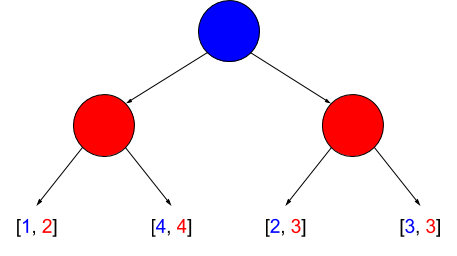
\includegraphics[scale = 0.4]{variable-sum-minimax-example.png}
\centering
\end{figure}

In the diagram above, there are just two players: Blue and Red.
The lists at the bottom represent terminal states of the game, in which the first number is Blue's points, and the second number is Red's points. ~\\

The Blue player can move Left or Right. 

If Blue takes the faithful approach, Blue thinks about what Red would do in each subgame, assuming that Red is rational.
If Blue were to move Left, then a rational Red would move Right, earning payoff [4, 4] for the players, and if Blue were to move Right, then a rational Red would assess Left and Right as equally favorable options, earning payoff [2, 3] or [3, 3] for the players.
After completing this analysis, Blue would decide to move Left, since doing so would lead to more points under the assumption of CKR. ~\\

In contrast, if Blue takes the conservative approach, what would Blue do?
If Blue moves Left, then the worst-case scenario earns 1 point, and if Blue moves Right, then the worst-case scenario earns 2 points.
Trying to make the best worst-case scenario, the conservative approach prescribes Right in this case. ~\\

The generalization of minimax that you will implement (for \verb|general_minimax| in the stencil) will take the conservative approach and choose a maximin action.

\subsection{Written Questions}
\begin{enumerate}
    \item The two approaches for generalizing minimax in variable-sum games in section 2.1.1 are both reasonable because they are both true of minimax in two-player, constant-sum games. ~\\
    Argue \textit{informally} that in two-player, constant-sum games, an action is a maximin actions if and only if it is the rational action to play under CKR.
    
    \item A friend says, ``Use the minimax algorithm if you can! It produces the best decisions possible in games.''
    Do you agree with their assertion?
    If not, give at least two reasons (not examples, but \textit{reasons}) why you think the assertion is wrong.
    Limit your response to 3 sentences.
    
\end{enumerate}



\section{The Code Files}
\subsection{Files to Modify}
\begin{itemize}
    \item \verb|adversarialsearch.py| is where you will complete the coding task.
\end{itemize}

\subsection{Necessary Source Code}
\begin{itemize}
    
    \item \verb|adversarialsearchproblem.py| contains two abstract classes: \\
    \verb|AdversarialSearchProblem| and \verb|GameState|. \\
    \verb|AdversarialSearchProblem| is analogous to \verb|SearchProblem| from the previous assignment; it contains methods that all adversarial search problems have in common.
    All of the algorithms that you will implement in this assignment take in an \verb|AdversarialSearchProblem|.
    The \verb|GameState| class is also abstract.
    It represents a game state.
    The only requirement of a game state that is imposed by the \verb|GameState| class is that a game state have some method of getting the player who will move next, and implement that method as the \verb|player_to_move| method. 
    The subclasses of \verb|AdversarialSearchProblem| are in \verb|gamedag.py| and \verb|tttproblem.py|.
    See them for specific examples of how this works.
\end{itemize}

\subsection{Optional Code for Testing}
\begin{itemize}
    \item \verb|gamedag.py| implements a generalization of a game tree---a game DAG (directed, acyclic graph)---as an \verb|AdversarialSearchProblem|.
    This helps you create simple, abstract adversarial search problems to make testing easier. Below is a visualization of the DAG created in the \verb|exampleDAG| function in \verb|adversarialsearch|. Running each of your functions on a DAG of this size should take no more than 1 second.
\begin{figure}[h]
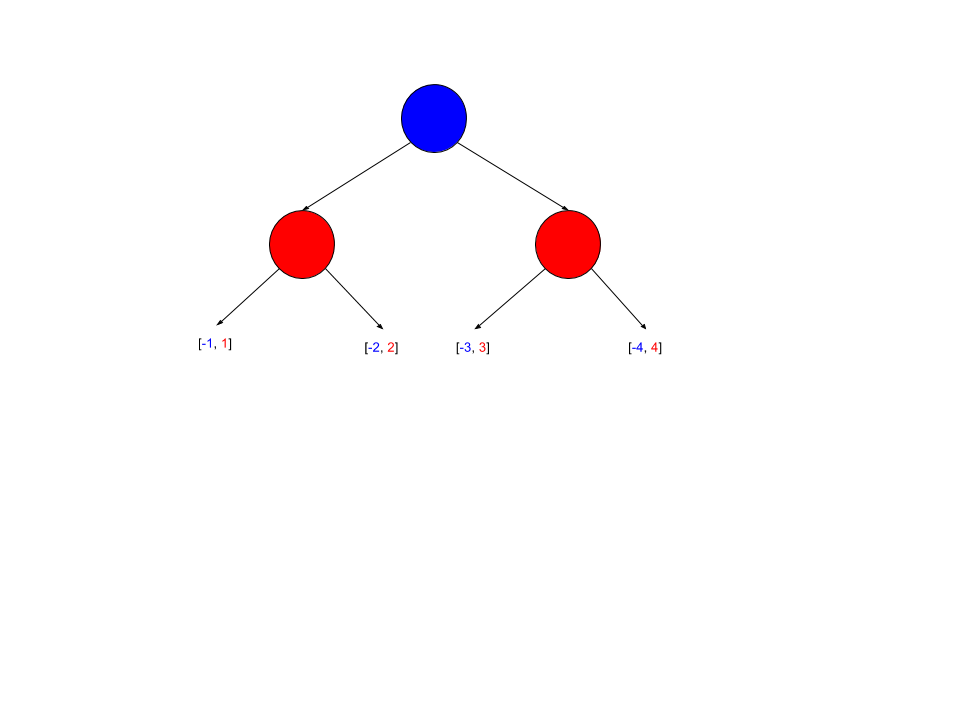
\includegraphics[scale = 0.4]{example-DAG.png}
\centering
\end{figure}
\end{itemize}


\subsection{Optional Code for Fun}
We have implemented TicTacToe as an implementation of \verb|AdversarialSearchProblem| for you.
It may be useful for sanity-checking your algorithms and understand ASPs, but it is mainly meant for fun, so that you can see
the algorithms come to life!
See the code file for details.
\begin{itemize}
\item \verb|tttproblem.py| includes the Tic-Tac-Toe game.
\item \verb|gamerunner.py| allows you to run and visualize games using your algorithms.
It's general enough that if you want to create a new game as an ASP, you can use \verb|gamerunner.py| to run it.
\end{itemize}

\section{Help}
You can find pseudocode for the minimax algorithm on page 166 of the textbook. 
You can find pseudocode for the alpha-beta pruning algorithm on page 170 of the textbook.
Note that you will need to modify the pseudocode significantly to work with \verb|AdversarialSearchProblem|s, but this should give you an idea about how the algorithms work. ~\\

Additionally, we have found \href{http://inst.eecs.berkeley.edu/~cs61b/fa14/ta-materials/apps/ab_tree_practice/}{\underline{this resource}} helpful for understanding alpha-beta pruning.

\section{Grading}

We will give you your score based on the rubric in \verb|rubric.txt|.

For both alpha\_beta and alpha\_beta\_cutoff, you will earn points for ``expands game states in a correct way."
To evaluate this, the autograder will look only at the sequence of (GameState, action) pairs on which \verb|transition(.)| is called.
What we're looking for here is that, in whatever order you visit the game states, you prune all the branches that you should when visiting in that order.

Avoid superfluous calls to \verb|transition(.)| they will throw off the auto-grader. 

\section{Install and Handin Instructions}
To install, run \verb|cs1410_install Adversarial_Search| from within your cs1410 directory. ~\\

To hand in, run \verb|cs1410_handin Adversarial_Search| from within your cs1410 directory. ~\\

In addition, please turn in the written portion of the assignment via Gradescope.


\end{document}
